\section{Pada Repo Lokal}
Semakin banyak yang bekerja maka semakin sering terjadi konflik. Sebagai contoh apabila dalam satu waktu atau satu hari ada empat orang melakukan penambahan atau pengurangan kode atau tulisan pada repo yang sama dan file yang sama, maka bisa dipastikan pasti akan terdapat konflik. Sehingga konflik merupakan hal yang biasa dan tidak perlu panik. Hanya kita harus mengetahui bagaimana melakukan solusi merge terhadap konflik tersebut. Karena satu satunya cara agar konflik bisa tersolusikan adalah dengan merge. Beberapa hal yang harus sering diperhatikan agar penyelesaian konflik tidak bikin kita pusing, antara lain :
\begin{itemize}
	\item sebelum melakukan pekerjaan pastikan sudah melakukan \textit{git pull origin master, git fetch upstream, git pull upstream master, git push origin master}.
	\item setelah menyelesaikan editing pada satu file, maka lakukan add dan commit hanya untuk satu file, hindari commit untuk beberapa file. jadi git add satufile, git commit apa yang dilakukan pada file tersebut. Jadi apabila ada dua file maka ada dua kali commit.
	\item sebelum melakukan \textit{pull request} pastikan juga sudah melakukan \textit{git pull origin master, git fetch upstream, git pull upstream master, git push origin master}.
\end{itemize}
Nah karena konflik adalah sebuah kepastian maka cara mengatasinya pun harus tepat. Pertama biasanya commit datang setelah melakukan \textit{git pull origin master, git fetch upstream, git pull upstream master, git push origin master}.
Biasanya akan muncul editor \textit{vi} seperti pada gambar \ref{fig:editorvimergesimpan} pada saat memasukkan perintah pull. Kita tinggal menyimpannya dengan menekan tombol esc, tombol :, tombol w, tombol q, tombol enter.

\begin{figure}[!htbp]
\centerline{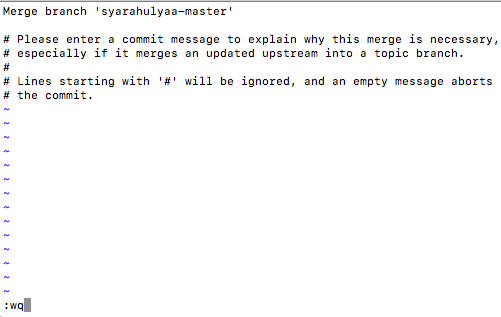
\includegraphics[width=.75\textwidth]{Figures/editorvimergesimpan}}
\caption{Muncul editor vi pada saat pull}
\label{fig:editorvimergesimpan}
\end{figure}

Baru setelah itu kita buka file yang konflik tersebut, sebagai contoh pada gambar \ref{fig:fileyangkonflik}. Perhatikan di gambar \ref{fig:fileyangkonflik} ada tulisan \textit{CONFLICT (content): Merge conflict in chapters/1.tex}.

\begin{figure}[!htbp]
\centerline{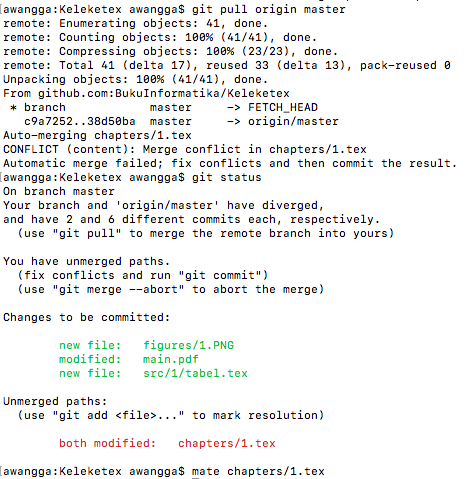
\includegraphics[width=.75\textwidth]{Figures/fileyangkonflik}}
\caption{Konflik Pada Saat \textit{git pull}}
\label{fig:fileyangkonflik}
\end{figure}

Artinya kita harus membuka file \textit{chapters/1.tex} karena ada konflik di dalamnya. Buka dengan editor kesukaan kita dan cari tanda konflik seperti pada gambar \ref{fig:konfliksebelum}. Perhatikan tugas kita adalah melakukan \textit{merge}, apa itu \textit{merge}? Merge adalah proses untuk melakukan penggabungan dari file atau baris yang telah di ubah dari beberapa versi yang konflik. Disini kita lihat bahwa pada gambar \ref{fig:konfliksebelum} ada tanda sama dengan sebagai pemisah antara versi satu dan versi dua dengan batas atas tanda kurang dari beberapa kali dan batas bawah lebih dari beberapa kali. Artinya kita harus menggabungkan hasil versi satu dan versi dua tersebut menjadi satu kesatuan sesuai dengan permintaan dari pemilik repo. Cara penggabungannya mau tidak mau suka atau tidak suka, kita baca manual dan perhatikan mana yang berbeda dan mana yang harus di sempurnakan kemudian di jadikan satu versi. Sehingga hasil penggabungan bisa dilihat pada gambar \ref{fig:konfliksesudah}, tentunya batas versi dari konflik sudah dihapus jangan sampai tertinggal karena pasti akan masih dianggap konflik. Dan bisa jadi bukan hanya ada satu konflik dalam satu file tersebut, kita harus mencarilagi batas konflik dua versi tersebut. Setelah selesai maka kita bisa menyimpan dan melakukan git add dan git commit.


\begin{figure}[!htbp]
\centerline{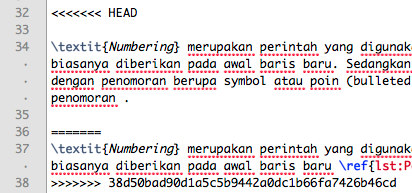
\includegraphics[width=.75\textwidth]{Figures/konfliksebelum}}
\caption{Tanda pembatas antara versi satu dan dua yang konflik}
\label{fig:konfliksebelum}
\end{figure}

\begin{figure}[!htbp]
\centerline{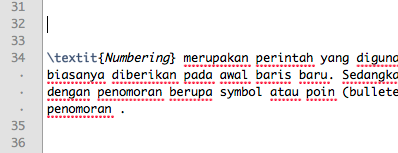
\includegraphics[width=.75\textwidth]{Figures/konfliksesudah}}
\caption{Konflik yang sudah diperbaiki menjadi satu versi baru lagi}
\label{fig:konfliksesudah}
\end{figure}


\section{Pada Saat Pull Request di Web}
Konflik yang terjadi pada web GitHub bagian ini biasanya terjadi pada saat melakukan pull request. Tertulis pada website ada konflik seperti gambar \ref{fig:webkonflik1}.

\begin{figure}[!htbp]
\centerline{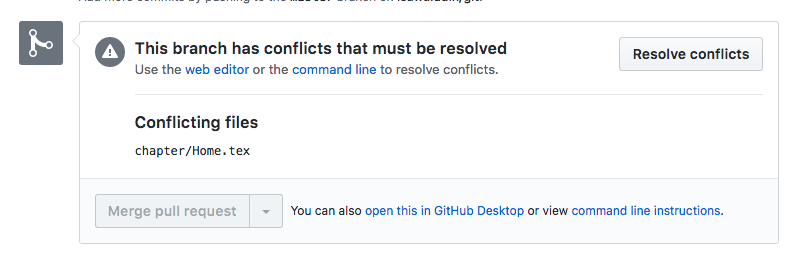
\includegraphics[width=.75\textwidth]{Figures/webkonflik1}}
\caption{Konflik Pada Saat Pull Request}
\label{fig:webkonflik1}
\end{figure}

Tetap tenang, ini sangatlah mudah untuk dilakukan solusinya yaitu dengan merge. Pertama kita klik Resolve conflicts yang terlihat pada gambar \ref{fig:webkonflik1}. Merge adalah proses memilih salah satu atau menggabungkan bagian yang ditandai oleh git. Sebagai contoh misalnya di gambar \ref{fig:webkonflik3}, tertulis ada 4 konflik.

\begin{figure}[!htbp]
\centerline{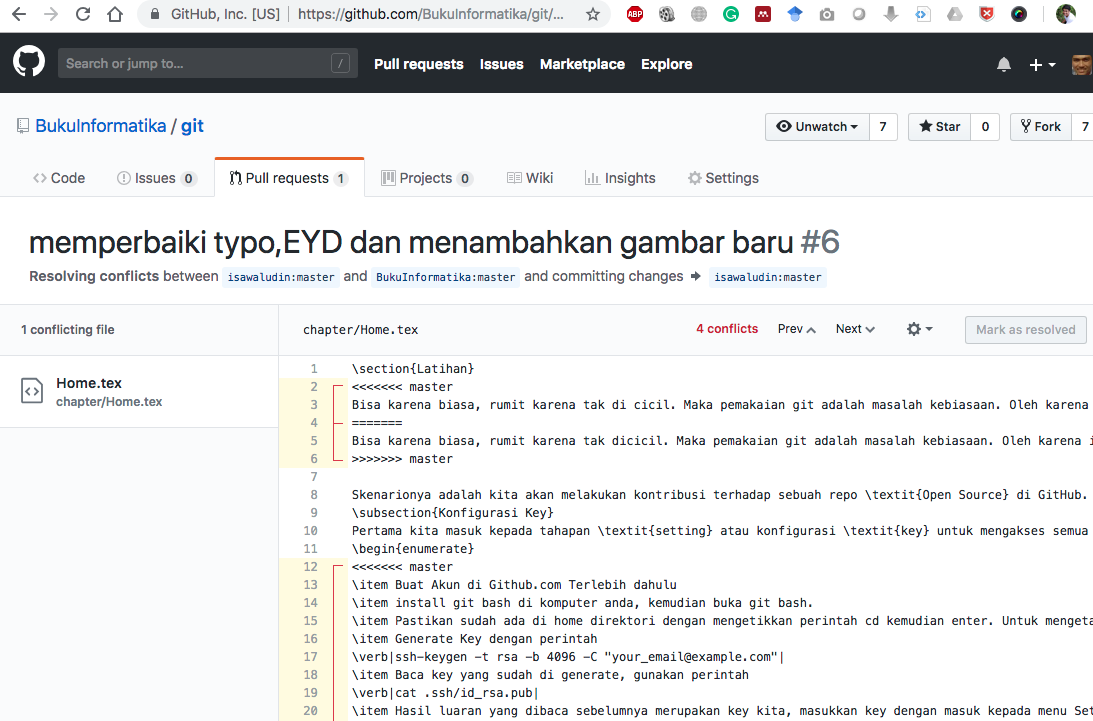
\includegraphics[width=.75\textwidth]{Figures/webkonflik3}}
\caption{Konflik Pada Saat Pull Request}
\label{fig:webkonflik3}
\end{figure}

Konflik yang pertama pada tulisan \textit{Bisa karena biasa....}. Maka kita tinggal melakukan merging dengan cara memilih kata pada baris ketiga atau kelima, atau bisa juga menggabungkan keduanya, jika memang isinya berbeda atau memodifikasi lagi. Setelah memilih jangan lupa menghapus tanda konflik seperti yang terlihat pada baris 2,4 dan 6. Baris 2 artinya itu tanda mulai, baris 6 artinya itu tanda akhir, dan baris 4 itu tanda untuk memilih apakah yang atas atau yang bawah. Sehingga definisi merge pada konflik ini terlihat pada gambar \ref{fig:webkonflik5}.



\begin{figure}[!htbp]
\centerline{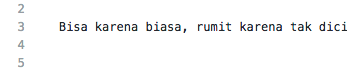
\includegraphics[width=.75\textwidth]{Figures/webkonflik5}}
\caption{Hasil Merge Setelah memilih dan menghapus tanda}
\label{fig:webkonflik5}
\end{figure}

\section{Lupa Compile dan Ingin Menambah Materi Lagi}
Bagaimana jika anda lupa meng-\textit{compile} padahal anda sudah melakukan tahap terakhir yaitu \textbf{git push origin master}. Ada solusi jitu untuk menanganinya tolong simak baik-baik ya.
\begin{enumerate}
  \item \textit{Compile} file \textbf{main.tex}, jika sudah selesai dan tanpa error anda kembali lagi ke gitbash.
  \item Inputkan perintah \textbf{git status} untuk memeriksa kembali apa saja yang belum kita tambahakan seperti pada gambar \ref{fig:status}.
      \begin{figure}[!htbp]
      \centerline{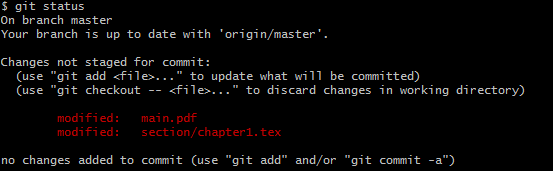
\includegraphics[width=.75\textwidth]{Figures/manajemenkonflik/status.png}}
      \caption{Memeriksa yang belum ditambahkan}
      \label{fig:status}
      \end{figure}
  \item Tambahkan file yang belum ditambahkan, seperti pada gambar \ref{fig:add}.
      \begin{figure}[!htbp]
      \centerline{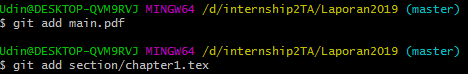
\includegraphics[width=.75\textwidth]{Figures/manajemenkonflik/add.png}}
      \caption{Menambahkan file}
      \label{fig:add}
      \end{figure}
  \item Melakukan proses pemeriksaan kembali untuk memastikan file yang ditambahkan sudah sesuai, seperti pada gambar \ref{fig:status1}.
      \begin{figure}[!htbp]
      \centerline{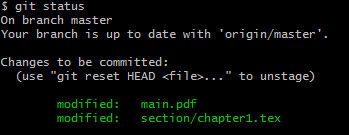
\includegraphics[width=.75\textwidth]{Figures/manajemenkonflik/status1.png}}
      \caption{Memastikan file yang sudah ditambah}
      \label{fig:status1}
      \end{figure}
  \item Melakukan proses \textit{Commit} seperti pada gambar \ref{fig:commit}.
      \begin{figure}[!htbp]
      \centerline{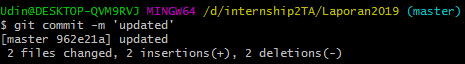
\includegraphics[width=.75\textwidth]{Figures/manajemenkonflik/commit.png}}
      \caption{Melakukan proses commit}
      \label{fig:commit}
      \end{figure}
  \item Nah ini adalah \textbf{Point Penting} yang selalu lupa untuk dilakukan yaitu melakukan perintah \textit{git pull upstream master}, mengapa harus melakukan hal tersebut? \textbf{Alasannya untuk menghindari terjadinya konflik dan memastikan bahwa repositori kita sudah up to date} seperti pada gambar \ref{fig:pull}.
      \begin{figure}[!htbp]
      \centerline{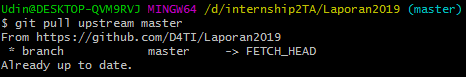
\includegraphics[width=.75\textwidth]{Figures/manajemenkonflik/pull.png}}
      \caption{Memastikan bahwa sudah up to date}
      \label{fig:pull}
      \end{figure}
  \item Step terakhir sudah pasti memasukkan perintah \textbf{git push origin master} seperti pada gambar \ref{fig:push}.
      \begin{figure}[!htbp]
      \centerline{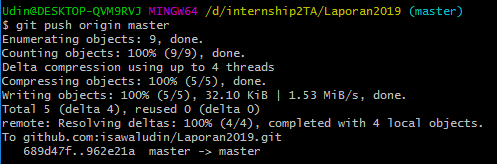
\includegraphics[width=.75\textwidth]{Figures/manajemenkonflik/push.png}}
      \caption{Step terakhir}
      \label{fig:push}
      \end{figure}
\end{enumerate}

\section{Bagaimana cara mudah dan cepat untuk memperbaiki error yang tidak terdeteksi}
Semakin banyak yang ikut berkontribusi di dalam sebuah repositori maka akan semakin sering menemui konflik, error merge dan permasalahan lainnya. Bagaimana solusinya jika tidak mengetahui error nya dimana. \textbf{Perhatikan dengan seksama ya}. Ini merupakan langkah yang tidak disarankan namun ampuh untuk menangani solusi.
\begin{enumerate}
\item Hapus repo lama di direktory masing-masing,
\item Buka git bash dan melakukan proses clone ulang dengan perintah \textbf{git clone LinkSSHdariRepo},
\item Lalu masukkan perintah \textbf{cd RepoygSudahdiDownload},
\item Remote kembali repo kita sesuaikan dengan repo asal dengan perintah \textbf{git remote add upstream LinkHttpsdariRepoAsal},
\item Lalu melakukan Fetch dengan perintah \textbf{git fetch upstream},
\item Melakukan Pull dengan perintah \textbf{git pull origin master},
\item Lakukan kembali perintah \textbf{git fetch upstream},
\item Melakukan Pull dengan perintah \textbf{git pull upstream master},
\item Maka akan muncul pemberitahuan errornya dimana, dan periksa di chapter/file yang sudah diberitahukan. Dan tinggal diperbaiki yang mana baris yang tidak selaras dan yang menimbulkan error merge dan error compile. \textbf{Selamat mencoba}.
\end{enumerate}
Ada pun cara lain jika Anda mengalami kejadian "\textit{Unable to Merge}" dan Anda kebingungan karena Anda sudah \textit{push} tetapi pada saat \textit{pull request} Anda tidak bisa melakukannya, cara ini mungkin dapat membantu Anda agar bisa melakukan \textit{pull request} (terutama file konflik nya ada di file PDF, akan sangat berguna menggunakan cara ini).
\begin{enumerate}
\item \textit{backup} dahulu yang sudah anda kerjakan. Tidak perlu \textit{backup} keseluruhan repo, cukup \textit{file} yang anda kerjakan,
\item Buka repo asal (misal BukuInformatika/git) dari pekerjaan yang Anda kerjakan (bukan repo hasil \textit{fork} kita sendiri),
\item \textit{Download ZIP, Extract} ke direktori lokal pekerjaan repo Anda,
\item Lakukan sinkronisasi dengan Repo asal untuk memastikan apakah masih ada \textit{error} ketika kita melakukan \textit{merge},
\item Jika tidak ada \textit{error}, maka, masukkan lagi pekerjaan yang sudah kita \textit{backup} tadi,
\item \textit{add file, commit, push},
\item Coba lagi melakukan \textit{Pull Request}, maka hasilnya akan menjadi ceklis hijau.
\end{enumerate}